% p:q
% Unofficial ERC Starting Grant LaTeX template 
% Source: http://www.arj.no/2013/02/03/erc-stg-latex/
%
\documentclass[oneside, a4paper, onecolumn, 11pt]{article}
%up to 15 pages without budget table and references
%%% PACKAGES %%%

\usepackage[left=2cm,top=2cm,bottom=1.5cm,right=2cm]{geometry}
\usepackage{hyperref}
\usepackage[utf8]{inputenc}
\usepackage{graphicx} 		% Add graphics capabilities
\usepackage{amsmath}  		% Better maths support
\usepackage{natbib}	% bibliography style
\setlength{\bibsep}{0.0pt}
\usepackage{eurosym}
\usepackage{comment}
\usepackage{floatrow}
\usepackage{afterpage}
\usepackage{color,xcolor}
\definecolor{absolutezero}{rgb}{0.0,0.28,0.73}
\definecolor{bluetiful}{rgb}{0.24,0.41,0.91}
\definecolor{aoenglish}{rgb}{0.0,0.5,0.0}
\definecolor{imperialred}{rgb}{0.93,0.16,0.22}
\usepackage{multirow}
\usepackage{colortbl}
\usepackage{lmodern,textcomp}
\usepackage{relsize} % e.g. used for \mathsmaller
\usepackage{caption}
\usepackage{array}
\usepackage{tikz}
\usetikzlibrary{fit,shapes, arrows}
\usepackage{chemfig}
\usetikzlibrary{decorations.markings}


\linespread{1.0}

% To fix list things: 
\usepackage{enumitem}
\setitemize{noitemsep,topsep=0pt,parsep=0pt,partopsep=0pt,leftmargin=*}
\usepackage{amssymb}
\renewcommand{\labelitemi}{\tiny$\blacksquare$}

\usepackage{nopageno}
\usepackage{enumitem}

\usepackage{fancyhdr}
\pagestyle{fancy}
\renewcommand{\headrulewidth}{0pt} % Remove line at top

\usepackage{todonotes}
\usepackage{subcaption}

 
\lhead{}
\rhead{}
\chead{\textbf{Exploring alternative formulations of Smoothed Particle Hydrodynamics for complex fluids and solids}}
\cfoot{\thepage}

\newenvironment{itemize*}%
  {\begin{itemize}%
    \setlength{\itemsep}{0pt}%
    \setlength{\parskip}{0pt}}%
  {\end{itemize}}

\renewcommand\thesection{\alph{section}}
%\renewcommand\thesubsection{\thesection.\arabic{subsection}}
\renewcommand\thesubsection{\thesection.\arabic{subsection}}
%\def\thesection{\arabic{subsection}}



\usepackage{enumitem}

%\renewcommand{\thesubsection}{\thesection.\alph{subsection}}
%\renewcommand{\thesubsection}{\Alph{subsection}}
\newcommand{\EE}{\mathbf{E}}
\newcommand{\DD}{\mathbf{D}}
\newcommand{\BB}{\mathbf{B}}
\newcommand{\HH}{\mathbf{H}}
\renewcommand{\AA}{\mathbf{A}}
\newcommand{\PP}{\mathbf{P}}
\newcommand{\ppi}{\boldsymbol{\pi}}
\newcommand{\oomega}{\boldsymbol{\omega}}
\newcommand{\MM}{\mathbf{M}}
\newcommand{\JJ}{\mathbf{J}}
\newcommand{\ii}{\mathbf{i}}
\newcommand{\vv}{\mathbf{v}}
\newcommand{\mm}{\mathbf{m}}
\newcommand{\xx}{\mathbf{x}}
\newcommand{\XX}{\mathbf{X}}
\newcommand{\yy}{\mathbf{y}}
\newcommand{\WW}{\mathbf{W}}
\newcommand{\diff}{\mathrm{d}}
\newcommand{\A}[2]{A^{\mathsmaller#1}_{\ \, #2}}
\newcommand{\nn}{\mathbf{n}}
\newcommand{\II}{\mathbf{I}}
\newcommand{\FF}{\mathbf{F}}
\newcommand{\QQ}{\mathbf{Q}}
\newcommand{\CC}{\mathbf{C}}
\renewcommand{\SS}{\mathbf{S}}
\newcommand{\eeta}{\boldsymbol{\eta}}
\renewcommand{\aa}{\mathbf{a}}
\newcommand{\qq}{\mathbf{q}}
\newcommand{\BBB}{\boldsymbol{\mathcal{B}}}
\newcommand{\dWW}{\mathrm{d}\mathbf{W}}
\newcommand{\OO}{\mathbf{1}}
\newcommand{\TT}{\mathbf{2}}
\newcommand{\intd}{\int\,\diff}
\newcommand{\rr}{\mathbf{r}}
\newcommand{\pp}{\mathbf{p}}
\newcommand{\LL}{\mathbf{L}}
\newcommand{\ee}{\mathbf{e}}

\renewcommand{\ss}{\mathbf{s}}

%%% COMMANDS %%%

\begin{document}
%%% Content

%\begin{center}
%\large{\textbf{
%ERC Starting Grant 2021\\
%Part B2}}
%\end{center}


%\begin{figure}[ht]
%    \centering
%    \includegraphics[scale=0.6]{corpse.jpg}
%    \caption{A galvanised corpse \citep{corpse}. As the usual parabolic equations for electrochemistry are purely dissipative, they inevitably monotonously approach their terminal state, thermodynamic equilibrium. On the other hand, hyperbolic electrochemistry (Inertial Electrochemistry) would be equipped with inertial effects allowing the systems to evolve no only irreversibly towards the equilibrium, but also reversibly.}
%\end{figure}
%\afterpage{\clearpage}

%\tableofcontents


%\end{enumerate}
\begin{center}
    \vspace*{\fill}
    {\Huge\bfseries Exploring alternative formulations of Smoothed Particle Hydrodynamics for complex fluids and solids}
    \vspace*{\fill}
\end{center}
\begin{center}
    \textbf{Michael Monček}\\
    % \vspace{0.5cm}
    % \textit{Mathematical Institute of Charles University, Prague, Czechia}\\
    % \vspace{0.5cm}
    \textbf{Supervisor:} \textbf{Michal Pavelka}\\
    % \vspace{0.5cm}
    % \textit{Mathematical Institute of Charles University, Prague, Czechia}\\
    % \vspace{0.5cm}
    % \textbf{Date:} May 14, 2025
\end{center}
%\clearpage

% I am applying for the Student Faculty Grant "Exploring alternative formulations of Smoothed Particle Hydrodynamics for complex fluids and solids" under the Mathematical Institute of Charles University.
% \vspace{\fill}
% \begin{itemize}

% \item \textbf{Applicant}: Michael Monček, $3^{\text{rd}}$ year Bachelor student of Mathematical Modelling, intending to continue with a Master’s degree in Mathematical Modelling in Physics and Technology at the Mathematical Institute of Charles University.



% \begin{figure}[H]
%     \centering
%     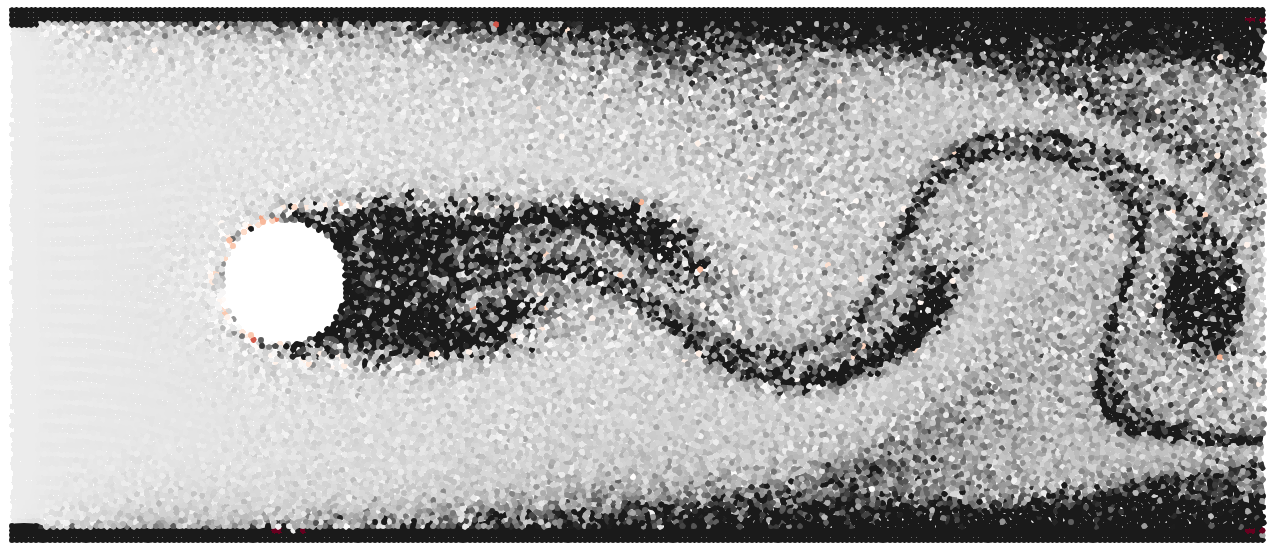
\includegraphics[width=0.85\linewidth]{distortion_grey_highres.png}
%     \caption{The distortion field in the flow around cylinder benchmark simulated using SHTC-SPH.}
%     \label{fig:enter-label}
% \end{figure}

% \item \textbf{Introduction}: Complex fluids and solids can be described by the Symmetric Hyperbolic Thermodynamically Compatible (SHTC) equations. These equations have a Hamiltonian structure and are advantageous in problems with large deformations and shock waves. One of the state variables in the SHTC equations is the distortion field (close to the inverse of the deformation gradient). Recently, a new numerical method solving the SHTC equations was developed based on the Smoothed Particle hydrodynamics (SPH) \cite{kincl-unified}. 

% However, in a later work \cite{hutter-pavelka}, an alternative definition of the discrete distortion that is useful when adding noise to the SHTC equations (to be applied in continuum physics of nanomaterials) was developed. In this definition, the discrete distortion is defined as the minimizer of the following functional, 
% \begin{equation*}
% 	D = \sum_\alpha\sum_\beta w_\alpha w_\beta ||\mathbf{R}_{\alpha\beta} - \mathbf{A} \cdot \mathbf{r}_{\alpha\beta}||^2,
% \end{equation*}
% where $\mathbf{R}_{\alpha\beta}$ is the difference between the Lagrangian positions of the particles $\alpha$ and $\beta$, $\mathbf{r}_{\alpha\beta}$ is the difference between Eulerian positions, and $w_\alpha(\mathbf{r})$ is a weight kernel of particle $\alpha$ (for instance the SPH kernel). The minimization of this functional leads to a discrete distortion field $\mathbf{A}$ that may be more suitable for SPH simulations of SHTC equations. 

% If the numerical SPH-based method becomes compatible with the new definition, it would be possible to simulate nanomembranes and other nanomaterials, where fluctuations play an important role, by the method. 

% 	\item \textbf{Goal}: 
% 	\begin{itemize}
% 	\item Reformulation of the numerical framework from \cite{kincl-unified} to the new definition of the distortion field.
% 	\item Comparison of the two formulations of the SHTC equations in SPH simulations.
% 	\end{itemize}


% \item \textbf{Specific tasks and Work Plan}: 
% \begin{enumerate}
% \item \textbf{July – December 2025}: %Use the definition of distortion from \cite{hutter-pavelka} to reformulate the SPH method from \cite{kincl-unified}.
% Reformulation of the SPH method to incorporate the new definition of distortion
% \item \textbf{July – December 2025}: As the formulation of the discrete dynamics in \cite{kincl-unified} is simplified, an attempt to use the full system of equations without neglecting the denominator of the discrete distortion matrix.

% \item \textbf{January – April 2026}: Comparative simulations of benchmark problems simulated in \cite{kincl-unified}, for instance the Beryllium plate benchmark or lid-driven cavity. 
% \item \textbf{April – May 2026}: If the tests are successful, extension to fluid-structure interaction problems
% (e.g. Turek-Hron bechmark \cite{turek-hron}).

% \item \textbf{May – July 2026}: Final analysis, documentation, and preparation of research output.
% \end{enumerate}

% \item \textbf{Project Duration}:
% \begin{itemize*}
% \item \textbf{Start Date}: July 1, 2025
% \item \textbf{End Date}: July 1, 2026
% \end{itemize*}

% \item \textbf{Relation to Bachelor’s Thesis}:
% The topic of this project is related to the applicant's Bachelor thesis, which concerns numerical simulation of
% fluid-structure interaction problems using the numerical method developed in \cite{kincl-unified}.
% The SFG project is designed to go beyond the scope of the thesis by exploring new formulations and applications.
% This project also serves as a foundation for future research in the applicant’s planned Master’s studies at the Mathematical Institute of Charles University.


% \item \textbf{Supervisor}: Michal Pavelka (Mathematical Institute of Charles University), pavelka@karlin.mff.cuni.cz

% \end{itemize}








% \vspace{2cm}

% \begin{tabular*}{\textwidth}{@{\extracolsep{\fill}} l r}
% Prague, May 14, 2025 & 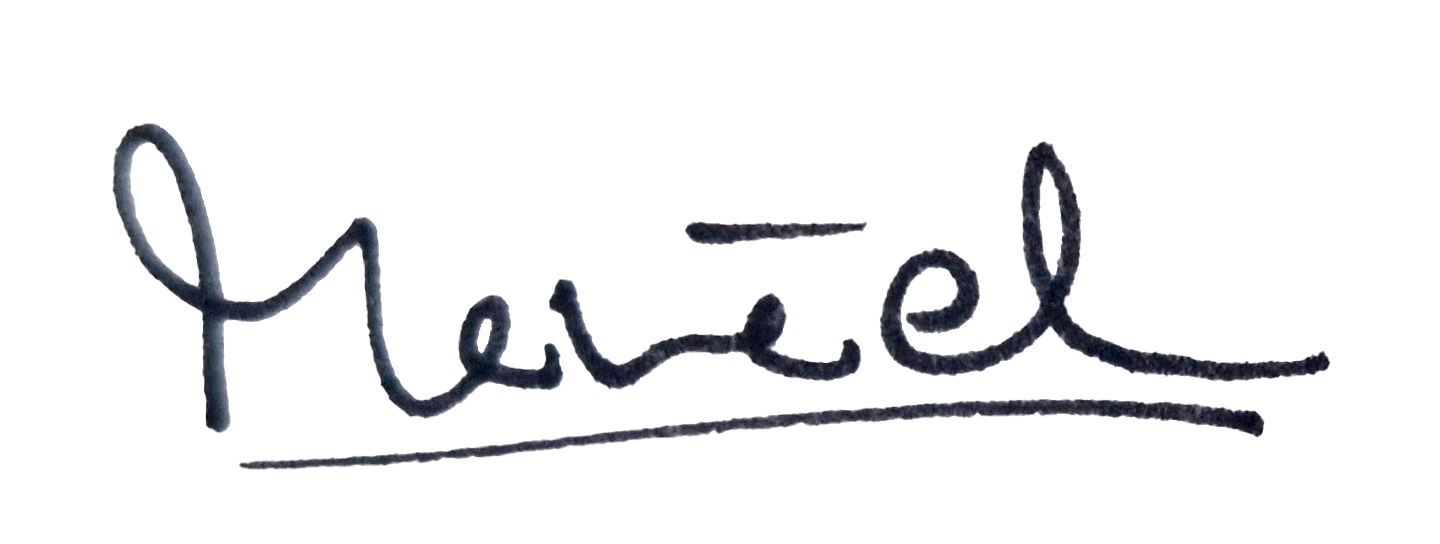
\includegraphics[height=1.5cm]{signature.png} \\
% & Michael Monček
% \end{tabular*}

\newpage
\begin{section}{Introduction}
   Complex fluids and solids can be described by the Symmetric Hyperbolic Thermodynamically Compatible (SHTC) equations. These equations have a Hamiltonian structure and are advantageous in problems with large deformations and shock waves. One of the state variables in the SHTC equations is the distortion field (close to the inverse of the deformation gradient). Recently, a new numerical method solving the SHTC equations was developed based on the Smoothed Particle hydrodynamics (SPH) \cite{kincl-unified}. 

However, in a later work \cite{hutter-pavelka}, an alternative definition of the discrete distortion that is useful when adding noise to the SHTC equations (to be applied in continuum physics of nanomaterials) was developed. In this definition, the discrete distortion is defined as the minimizer of the following functional, 
\begin{equation*}
    D_{\xx}(\AA) = \sum_a \sum_b w_a(\xx) w_b(\xx) \| \XX_{ab} - \AA(\xx) \xx_{ab} \|^2
\end{equation*}
where $\XX_{ab}$ is the difference between the Lagrangian positions of the particles $a$ and $b$,
$\xx_{ab}$ is the difference between Eulerian positions, and $w_a(\xx)$ is a weight kernel of particle $a$ (for instance the SPH kernel) and $\AA(\xx)$ is a matrix representation
of the distortion field.

This approach is a counterpart to the one used in \cite{kincl-unified} as we are not evolving the distortion field in time according to the SHTC equations 
but rather defining it as a minimizer of the functional above at each time step. 
An advantage of this approach is that it in theory it is possible to add fluctuations to the model, which would enable us to simulate nanomembranes and other nanomaterials, where 
fluctuations play a crucial role. 


% The minimization of this functional leads to a discrete distortion field $\mathbf{A}$ that may be more suitable for SPH simulations of SHTC equations. 

% If the numerical SPH-based method becomes compatible with the new definition, it would be possible to simulate nanomembranes and other nanomaterials, where fluctuations play an important role, by the method. 
\end{section}

\begin{section}{Methods}
\begin{itemize}
    \item distortion as an error estimator (compare different definitions)
    \item comparison with Ondra's SPH
\end{itemize}
\begin{subsection}{Distortion as a minimization problem}
    In this section we will define the distortion field as a minimizer of the following minimization problem:
    \begin{equation}\label{ls_problem}
        \AA(x) = \underset{\AA \in \mathbb{R}^{d\times d}}{\text{argmin}} \sum_b w(\xx - \xx_b) \| \AA(\xx - \xx_b) - (\XX - \XX_b)\|^2
    \end{equation}
    The term
    \begin{equation}
    e_{b}(\xx) := \|\AA(\xx - \xx_b) - (\XX - \XX_b)\|
    \end{equation}
    plays the role of the error by which we fail to approximate the linearized relation:
     \begin{equation}
        \AA(x) d\xx - d\XX = 0
    \end{equation}
    The equation \Ref{ls_problem} can be than written compactly as:

    \begin{equation}
        \AA(x) =  \underset{\AA \in \mathbb{R}^{d\times d}}{\text{argmin}} \sum_{b} w(\xx - \xx_b) e_b(\xx)^2 
    \end{equation}
    which is a weighted least squares problem. 
    
    Evaluated at position $\xx_a$ associated with particle $a$ we get the following:
    \begin{equation}
        \AA_{a} = \underset{\AA \in \mathbb{R}^{d\times d}}{\text{argmin}} \sum_{b} w_{ab} \|\AA \xx_{ab} - \XX_{ab}\|^2
    \end{equation}

    Next we will prove that \Ref{ls_problem} has a solution:
    \newtheorem{LS_problem}{Lemma: (LS problem)}

    \begin{LS_problem}
        \text{The LS problem } \Ref{ls_problem} \text{ has a solution.}
    \end{LS_problem}
    \textbf{Proof:}\\
    Let $I(\AA_a) :=  \frac{1}{2} \sum_{b} w_{ab} |\ \AA_{a}\xx_{ab} - \XX_{ab}\|^2$ and observe that 
    $I(\AA_a)$ is a differentiable and coercive function meaning: 
    \begin{equation}
        I(\AA_a)/\|\AA_a\| \rightarrow + \infty
    \end{equation}
    This implies existence of global minimum. %The neccessary condition for existence of a min 
    
    We can also compute this minimum explicitely:\\
    Lets denote $\AA_{a}\xx_{ab} - \XX_{ab} =: e_{ab}$ and lets take the Gatteaux derivative of $I(\AA_a)$ in the direction $\diff \AA_a$
    \begin{equation}
        \begin{aligned}
        \text{D}I(\AA_{a})[\diff \AA_a] := \lim_{\lambda \rightarrow 0+} 
        \frac{I(\AA_{a} + \lambda \diff \AA_a) - I(\AA_a)}{\lambda} =\\ 
        \lim_{\lambda \rightarrow 0+} \sum_{b} w_{ab} \left[ 
        \left( e_{ab} + \lambda \diff \AA_a \xx_{ab}, e_{ab} + 
        \lambda \diff \AA_a \xx_{ab} \right) - \left( e_{ab}, e_{ab} \right) \right] = \\
        \lim_{\lambda \rightarrow 0+} \frac{1}{2\lambda} \sum_{b}w_{ab} \left( 2(e_{ab}, \lambda \diff \AA_a \xx_{ab}\right) +
        \lambda^{2} \left( \diff \AA_{a} \xx_ab, \diff \AA_{a} \xx_ab \right)  =\\
        \sum_{b} w_{ab} \left( \AA_{a}\xx_{ab} - \XX_{ab} \right) \cdot \diff \AA_{a} \xx_{ab} = \\
        \diff \AA_{a} : \left( \sum_{b} w_{ab} \left( \AA_{a} \xx_{ab} - \XX_{ab} \right) \cdot \xx_{ab}  \right) 
        \end{aligned}
    \end{equation}
    Which immediately implies:
    \begin{equation}
        \AA_a = \PP_a \QQ_a^{-1}
    \end{equation}
    where \begin{equation}
        \PP_a = \left( \sum_b w_{ab} \XX_{ab} \otimes \xx_{ab} \right) \text{ and }
        \QQ_a =  \left( \sum_b w_{ab} \xx_{ab} \otimes \xx_{ab} \right)
    \end{equation}
    Notice that the matrix $\QQ_a$ is positive definite and hence invertible (unless $\xx_{ab} = 0$ for all $a, b$).
    To prove it, we need to show that $\vv \cdot \QQ_{a} \vv > 0 $ for each  nonzero $\vv$.
    \begin{equation}
        \vv \cdot \QQ_{a} \vv = \vv \cdot  \left( \sum_b w_{ab} \xx_{ab} \otimes \xx_{ab} \right) \vv =
        \sum_{b} w_{ab} (\xx_{ab} \cdot \vv)^2 > 0
    \end{equation}
    

    We can also generalize this and use the definition from Pavelka \& Hutter \cite{hutter-pavelka} where we hope to
    achieve better precision at the cost of summing over all particle pairs instead of singletons.
    \begin{equation}
        \AA^{double}(x) = \underset{\AA \in \mathbb{R}^{d\times d}}{\text{argmin}} \sum_b \sum_{c} w(\xx - \xx_b) w(\xx - \xx_c)
        \| \AA\xx_{bc} - \XX_{bc}\|^2
    \end{equation}
    Evaluated at position $\xx_a$ associated with particle $a$ we get the following: 
    \begin{equation}
        \AA^{double}_a = \underset{\AA \in \mathbb{R}^{d\times d}}{\text{argmin}} \sum_b \sum_{c} w_{ab} w_{ac}
        \| \AA\xx_{bc} - \XX_{bc}\|^2
    \end{equation}
    Following the same procedure as in the first example we get the explicit formula for 
    $\AA^{double}$ in this case:
    \begin{equation}
        \AA^{double}(\xx) = \left( \sum_{a,b} w_a w_b \XX_{ab} \otimes \xx_{ab} \right) 
        \left( \sum_{a,b} w_a w_b \xx_{ab} \otimes \xx_{ab} \right)^{-1}
    \end{equation} 
    Evaluated at position $\xx_a$ associated with particle $a$ we get the following:
    \begin{equation}
        \AA^{double}_a = \PP^{double}_a (\QQ^{double}_a)^{-1}
    \end{equation}
    where
    \begin{equation}
        \PP^{double}_a = \left( \sum_{b,c} w_{ab} w_{ac} \XX_{bc} \otimes \xx_{bc} \right) \text{ and } 
        \QQ^{double}_a = \left( \sum_{b,c} w_{ab} w_{ac} \xx_{bc} \otimes \xx_{bc} \right)
    \end{equation} 
    % To deal with the computational complexity that is quadratic in this case we can make the following observation:
    We can make the following interesting observation that allows us to rewrite $\AA^double_{a}$ in an alternative way:

    \textbf{Notice:} 
    \begin{equation}
        \xx_{bc} \otimes \xx_{bc} = (\xx_{b} - \xx_{c}) \otimes (\xx_{b}- \xx_c) =
        \xx_{b} \otimes \xx_{b} + \xx_{c} \otimes \xx_{c} - \xx_{b} \otimes \xx_{c} - \xx_{c} \otimes \xx_b
    \end{equation}
    Therefore we have:
    \begin{equation}
        \begin{aligned}
        \QQ^{double}_a = \sum_{b,c} w_{ab} w_{ac} \left( 
        \xx_{b} \otimes \xx_{b} + \xx_{c} \otimes \xx_{c} - \xx_{b} \otimes \xx_{c} - \xx_{c} \otimes \xx_b \right) =\\
        2 \left( \sum_{b} w_{ab} \right) \left( \sum_{b} w_{ab} \xx_{b} \otimes \xx_{b} \right) 
        - 2 \left( \sum_{b} w_{ab} \xx_b \right) \otimes \left( \sum_{b} w_{ab} \xx_b \right)
        \end{aligned}
    \end{equation}
    which after introducing the notation: $\bar \xx_{a} := (\sum_{b} w_{ab} \xx_b) / (\sum_{b} w_{ab})$ and realizing that
    $\sum_{b} w_{ab} (\xx_{b} - \bar \xx_a) = 0$ can be written as:
    \begin{equation}
        \QQ^{double}_a = 2 \left( \sum_{b} w_{ab} \right) \left( \sum_{b} (\xx_{b} - \bar \xx_a) \otimes  (\xx_{b} - \bar \xx_a) \right) 
    \end{equation}
    And similarly:
    \begin{equation}
        \PP^{double}_a = 2 \left( \sum_{b} w_{ab} \right) \left( \sum_{b} (\XX_{b} - \bar \XX_a) \otimes  (\xx_{b} - \bar \xx_a) \right) 
    \end{equation}
    We can also get rid of the prefactor $2 \left( \sum_{b} w_{ab} \right)$ as it will not change the value of $\AA^{double}_a$ 
    and simply write:
    \begin{equation}
        \AA^{double}_a = \left( \sum_{b} (\XX_{b} - \bar \XX_a) \otimes  (\xx_{b} - \bar \xx_a) \right)
        \left( \sum_{b} (\xx_{b} - \bar \xx_a) \otimes  (\xx_{b} - \bar \xx_a) \right)^{-1}
    \end{equation}
    Notice that to compute $\AA^{double}_a$ from this definition we only need to know 
    $\bar \xx_{a} := (\sum_{b} w_{ab} \xx_b) / (\sum_{b} w_{ab})$ which can be precomputed.
    
    Next we will make an observation about the order of approximation of $\AA_{a}$ and $\AA^{double}_a$:
    Lets start with the following taylor expansion:
    \begin{equation}
        \XX_{b} = \XX_{a} + \AA(\xx_a) \xx_{ba} + \frac{1}{2} \nabla \AA(\xx_a) [\xx_{ba}, \xx_{ba}] + O(h^3)
    \end{equation}
    we can plug it in the definition of $\PP_a$ to get:
    \begin{equation}
        \begin{aligned}
        \PP_{a} = \sum_{b} w_{ab} \left( \AA(\xx_a) \xx_{ba} + 
        \frac{1}{2} \nabla \AA(\xx_a) [\xx_{ba}, \xx_{ba}] + O(h^3) \right) \otimes \xx_{ab} = \\
        \AA(\xx_a) \left( \sum_{b} w_{ab} \xx_{ab} \otimes \xx_{ab} + O(h^3) \right) = 
        \AA(\xx_a) \QQ_{a} + O(h^3)
        \end{aligned}
    \end{equation}
    And finally from the definition of $\AA_a$ and using the fact that $\QQ_a^{-1} = O(h^2)$ we get:
    \begin{equation}
        \AA_{a} = \PP_{a} \QQ_a^{-1} = \left( \AA(\xx_a) + O(h^3) \right) \QQ_a^{-1} = \AA(\xx_a) + O(h)
    \end{equation}
   
    For $\AA^{double}$ we can proceed similarly 
    (using the notation $\nabla \AA^{double}(\xx_a) =: \mathbf{H}(\xx_a)$):
    \begin{equation}
        \begin{aligned}
            \XX_{ba} = \AA(\xx_a) \xx_{ba} + \frac{1}{2} \mathbf{H}(\xx_a)[\xx_{ba}, \xx_{ba}] + O(h^3) \\ 
            \XX_{ca} = \AA(\xx_a) \xx_{ca} + \frac{1}{2} \mathbf{H}(\xx_a)[\xx_{ca}, \xx_{ca}] + O(h^3) 
        \end{aligned}
    \end{equation}
    taking the difference of these two expansions we get:
    \begin{equation}
            \XX_{bc} = \AA(\xx_a) \xx_{bc} + \frac{1}{2} \left( \mathbf{H}(\xx_a)[\xx_{ba}, \xx_{ba}]
            - \mathbf{H}(\xx_a)[\xx_{ca}, \xx_{ca}] \right) + O(h^3)  
    \end{equation}
    pluggin this in the definition of $\PP^{double}_a$ and swapping the indecees in the last step we get:
    \begin{equation}
        \begin{aligned}
        \PP^{double}_a = \left( \sum_{b,c} w_{ab} w_{ac} \AA(\xx_a) \xx_{bc} \otimes \xx_{bc}
        + w_{ab} w_{ac} \frac{1}{2} \left( \mathbf{H}(\xx_a)[\xx_{ba}, \xx_{ba}]
            - \mathbf{H}(\xx_a)[\xx_{ca}, \xx_{ca}] \right) \otimes \xx_{bc} \right) + O(h^4) = \\
            \AA(\xx_a) \QQ_a^{double} + \sum_{b,c} w_{ab} w_{ac} \frac{1}{2} 
            \left( \mathbf{H}(\xx_a)[\xx_{ba}, \xx_{ba}]
            - \mathbf{H}(\xx_a)[\xx_{ca}, \xx_{ca}] \right) \otimes \xx_{bc} + O(h^4) =
            \AA(\xx_a) \QQ_a^{double} + O(h^4)
        \end{aligned}
    \end{equation}
    Finally we get:
    \begin{equation}
        \AA^{double} = \PP^{double}_a (\QQ^{double}_a)^{-1} = \AA(\xx_a) + O(h^2)
    \end{equation}
    
     

    
    
    \newtheorem{MLS_problem}{Lemma: (MLS problem)}
    
\end{subsection}

\begin{subsection}{Particle distortion field}
%     While it is possible to take the minimizer of the functional $D_{\xx}(\AA)$ directly resulting in 
% the distortion field $\AA$ defined as:
% \begin{equation}
%     \AA(\xx) = \left( \sum_{a,b} w_a w_b \XX_{ab} \otimes \xx_{ab} \right) 
%     \left( \sum_{a,b} w_a w_b \xx_{ab} \otimes \xx_{ab} \right)^{-1}
% \end{equation} 
% as suggested in Pavelka et al. \cite{hutter-pavelka}. It is worth noticing that in a particle method such as SPH,
% this definition becomes computationally expensive as it requires to sum over all particle pairs 
% $(a,b)$ in $\text{supp }w_a(\xx) \cap \text{supp }w_b(\xx)$.
%
% To alleviate this issue, we can slighlty modify this definition by considering only the diagonal terms of the weight kernels
% resulting in the following definition of the distortion field $\AA_a$ at point $\xx_a$ occupied by particle $a$ that is still 
% fully compatible with the SHTC equations under the same assumptions as in \cite{hutter-pavelka}:
 
% In our alternative formulation, the distortion field $\AA$ at point $\xx$ is defined as a minimizer of the following functional:
% \begin{equation}
%     D_{\xx}(\AA) = \sum_a \sum_b w_a(\xx) w_b(\xx) \| \XX_{ab} - \AA \xx_{ab} \|^2
% \end{equation}
% where $w_a(\xx) = w(\xx - \xx_a)$ and $\|\vv\|^2 = \vv \cdot \vv$ is the standard vector product.\\

% Evaluating the sufficient condition for the minimum of $D_{\xx}(\AA)$ yields:
% \begin{equation}
%     \frac{\diff D_{\xx}(\AA)}{\diff \AA} = \frac{\diff}{\diff\AA} \sum_a \sum_b w_a(\xx) w_b(\xx) \left( \XX_{ab} - \AA \xx_{ab} \right)^T \left( \XX_{ab} - \AA \xx_{ab} \right) =
%     \sum_a \sum_b w_a(\xx) w_b(\xx) \frac{\diff}{\diff \AA} \left(
%     \right)
% \end{equation}
% \begin{subsection} {Time evolution of the distortion field}
% \begin{equation}
%     \AA_a = \PP_a \QQ_a^{-1}
% \end{equation}
% where \begin{equation}
%     \PP_a = \left( \sum_b w_{ab} \XX_{ab} \otimes \xx_{ab} \right) \text{ and }
%     \QQ_a =  \left( \sum_b w_{ab} \xx_{ab} \otimes \xx_{ab} \right)
% \end{equation}
In this section we will compute the differential of the distortion field wrt a small perturbation in particle possition. 
Utilizing the definition of $\AA_a$ the differential of the distortion field with respect to position $\xx_a$ is then equal to:
\begin{equation}
    \diff \AA_a = \diff \PP_a \QQ_a^{-1} + \PP_a \diff \QQ_a^{-1} =
    \diff \PP_a \QQ_a^{-1} - \PP_a \QQ_a^{-1} \diff \QQ_a \QQ_a^{-1} 
\end{equation}
Which under the assumptions from \cite{hutter-pavelka}:
\begin{equation}
    \dot{\xx}_a \approx \dot{\xx}_b + \nabla \vv \Big|_{\xx_a} \cdot \xx_{ab} \text{ and } 
    \XX_{ab} \approx \AA_a \xx_{ab}
\end{equation} 
simplifies to: 
\begin{equation}
    \diff \AA_a = - \AA_a \nabla \vv(\xx) \Big|_{\xx_a}% = - \AA_a \LL_a 
\end{equation}
giving us the evolution equation for the distortion field
which is the evolution equation for the distortion field in the SHTC equations.\\
Computing $\diff \AA_a$ directly without any approximations yields:
\begin{equation}\label{eq:dA_full}
    \begin{aligned}
    \diff \AA_a = - \AA_a \LL_a +
    \left(\sum_b \nabla w_{ab} \cdot \diff \xx_{ab} \left(\XX_{ab} - \AA_a \xx_{ab}
    \right) \otimes \xx_{ab}\right)\QQ_a^{-1} +\\
    \left(\sum_b w_{ab} \left(\XX_{ab} - \AA_a \xx_{ab}
    \right) \otimes \diff \xx_{ab}\right)\QQ_a^{-1}
    \end{aligned}
\end{equation}
where:
\begin{equation}
    \LL_a := \left( \sum_b w_{ab} \vv_{ab} \otimes \xx_{ab}\right)
    \left( \sum_b w_{ab} \xx_{ab} \otimes \xx_{ab}\right)^{-1}
\end{equation}
and it can be seen as an SPH approximation of the velocity gradient at point $\xx_a$.
If we neglect the terms containing $\XX_{ab} - \AA_a \xx_{ab}$ this reduces to:
\begin{equation}\label{eq:dA}
    \diff \AA_a = - \AA_a \LL_a%\left( \sum_b w_{ab} \diff \xx_{ab} \otimes \xx_{ab}\right)
%    \left( \sum_b w_{ab} \xx_{ab} \otimes \xx_{ab}\right)^{-1}
\end{equation}
It remains to see whether this approximation is justified in practice, which we will discuss later.

\end{subsection}
\begin{subsection} {Equations of motion}
    In this section we will derive the equations of motion using equations \ref{eq:dA} and \ref{eq:dA_full}.

First let $U_h = \sum_b \epsilon_b$ be the total energy of the particle system, let $\epsilon_b$ be the specific energy 
density of particle $b$. We assume that the specific energy density depends on the density $\rho$ and the 
distortion field $\AA$ ie. $\epsilon_b = \epsilon_b(\rho_b, \AA_b)$. Using \ref{eq:dA} we can calculate the differential of the energy $U_h$ as: 
\begin{equation}
    \begin{aligned} 
    \diff U_h = \sum_a m_a \epsilon_{\AA_a} : \diff \AA_a + \sum_a m_a \epsilon_{\rho_a} \diff \rho_a
    = \sum_a m_a \epsilon_{\rho_a} \left( \sum_b m_b \diff \xx_{ab} \cdot \nabla w_{ab} \right)
    + \sum_a m_a \epsilon_{\AA_a} : \left( - \diff \AA_a \right) \\
    = \sum_{a,b} m_a m_b  \left( \epsilon_{\rho_a} \nabla w_{ab} \cdot \diff 
    \xx_{ab} - \frac{1}{m_b} \epsilon_{\AA_a} : \AA_a 
    \left( w_{ab} \diff \xx_{ab} \otimes \xx_{ab}\right) \QQ_a^{-1}
    \right) \\
    = -\sum_{a,b} m_a m_b \left(\frac{1}{m_b} w_{ab} \Pi_a \xx_{ab} - 
    \epsilon_{\rho_a} \nabla w_{ab}  \right) \cdot \diff \xx_{ab}\\
    = -\sum_{a,b} m_a m_b \left(\frac{1}{m_b} w_{ab} \Pi_a \xx_{ab} - 
    \epsilon_{\rho_a} \nabla w_{ab}  \right) \cdot \left(\diff \xx_a - \diff \xx_b\right)\\
    = -\sum_{a,b} m_a m_b \left(\frac{1}{m_b} w_{ab} \Pi_a \xx_{ab} - 
    \epsilon_{\rho_a} \nabla w_{ab}  \right) \cdot \diff \xx_a \\
    - \sum_{b,a} m_b m_a \left(\frac{1}{m_a} w_{ba} \Pi_b \xx_{ab} - 
    \epsilon_{\rho_b} \nabla w_{ab}  \right) \cdot \diff \xx_a\\ 
    = -\sum_{a,b} m_a m_b \left[ w_{ab} \left( \frac{\Pi_a}{m_b} + \frac{\Pi_b}{m_a} \right) \xx_{ab} 
    - \left( \epsilon_{\rho_a} + \epsilon_{\rho_b} \right) 
    \nabla w_{ab} \right] \cdot \diff \xx_a
    \end{aligned}
\end{equation} where $\Pi_a = \AA_a^T \epsilon_{\AA_a} \QQ_a^{-T}$.\\ 
Using Newton's second law $m \dot{\vv} = - \frac{\diff U}{\diff \xx}$ we get the following equations of motion: 
\begin{equation} 
    m_a \dot{\vv}_a = \sum_b m_a m_b \left[ w_{ab} \left( \frac{\Pi_a}{m_b} + \frac{\Pi_b}{m_a}\right) 
    \xx_{ab} - \left( \epsilon_{\rho_a} +
    \epsilon_{\rho_b} \right) \nabla w_{ab} \right] 
\end{equation} 
%{
% \todo[inline]{These equations are different from the equations Ondra originally proposed
%  and from those in the example code rod.jl something is wrong here.} 

Let us assume that the inner energy $\epsilon$ decomposes into bulk and shear part as $\epsilon(\rho, \AA) = 
\epsilon_0(\rho) + \epsilon_s(\AA)$. 
We will use the following quadratic relation for the bulk component:
\begin{equation}
    \begin{aligned}
    \epsilon_0(\rho) = c_0^2 / 2 \left(\frac{\rho_0}{\rho} - 1\right)^2\\
    \epsilon_0'(\rho) = c_0^2 \left(\frac{\rho_0}{\rho} - 1\right)
    \left(- \rho_0 / \rho^2 \right) = c_0^2 \rho_0 \left( \frac{1}{\rho^2}
    - \frac{\rho_0}{\rho^3}\right)
    \end{aligned}
\end{equation}
For the shear component we will use the following equation:
\begin{equation}
    \begin{aligned}
    \epsilon_s(\AA) = \frac{c_s^2}{4}\| \text{dev}(\AA^T\AA) \|^2_F\\
    \epsilon_s'(\AA) = c_s^2 \AA \text{dev}(\AA^T\AA)
    \end{aligned}
\end{equation}
We can than write the $\Pi_a$ as:
\begin{equation}
    \Pi_a = c_s^2 \AA^T_a \AA_a \text{dev}(\AA_a^T \AA_a) \QQ_a^{-T} 
\end{equation}

We can treat the density $\rho$ in two ways. The first one is the standard SPH density approximation:
\begin{equation}
    \rho_a = \sum_b m_b w_{ab}
\end{equation}
The second way is the following relation:
\begin{equation}
    \rho_a = \rho_0 \det(\AA_a)
\end{equation}

With this we have derived the following system of equations for the 
Particle distortion SPH-SHTC:

\begin{subequations}
    \begin{equation}
        \dot{\xx}_a = \vv_a\\
    \end{equation}
    \begin{equation}
        \dot{\vv}_a = \sum_b m_b \left[ w_{ab} \left( \frac{\Pi_a}{m_b} + 
        \frac{\Pi_b}{m_a}\right) \xx_{ab} - \left( \epsilon_{\rho_a} +
        \epsilon_{\rho_b} \right) \nabla w_{ab} \right]\\
    \end{equation}
    \begin{equation} 
        \AA_a = \left( \sum_b w_{ab} \XX_{ab} \otimes \xx_{ab} \right) 
        \left( \sum_b w_{ab} \xx_{ab} \otimes \xx_{ab} \right)^{-1}
    \end{equation}
\end{subequations}

THe only thing to see now is whether is works or not xD 
We have neglected some terms so here they are (using the notation $
\ee_{ab} = \XX_{ab} - \AA_a \xx_{ab}$):

\begin{equation}
    \sum_a m_a \epsilon_{\AA_a} :
    \left(\sum_b w_{ab} \ee_{ab} \otimes \diff \xx_{ab}\right)\QQ_a^{-1} =
    \sum_{a,b} w_{ab} \left(m_a \Pi'_a \ee_{ab} - 
    m_b \Pi'_b \ee_{ba}\right) \cdot \diff \xx_a
\end{equation}

\begin{equation}
    \sum_a m_a \epsilon_{\AA_a} :
    \left(\sum_b \nabla w_{ab} \cdot \diff \xx_{ab} 
    \ee_{ab} \otimes \xx_{ab}\right)\QQ_a^{-1}
    = \sum_{a,b} \left( \left(m_a \Pi'_a \ee_{ab} - m_b \Pi'_b \ee_{ba}\right) 
    \cdot \xx_{ab}\right) \nabla w_{ab} \cdot \diff \xx_a
\end{equation}

where $\Pi'_a = c_s^2 \QQ_a^{-1} \text{dev}(\AA_a^T \AA_a) \AA_a^T$ also note that
$\Pi_a = (\Pi'_a \AA_a)^T$ furthemore we will write 
$\ss_{ab} = \left(m_a \Pi'_a \ee_{ab} - m_b \Pi'_b \ee_{ba}\right)$.

The full form of the evolution equation for velocity then reads:
\begin{equation}
    \dot{\vv}_a = \sum_b m_b \left[ w_{ab} \left( \frac{\Pi_a}{m_b} + 
    \frac{\Pi_b}{m_a}\right) \xx_{ab} - \left( \epsilon_{\rho_a} +
    \epsilon_{\rho_b} \right) \nabla w_{ab} - 
    \left( w_{ab} \frac{1}{m_a m_b} \ss_{ab} + 
    \ss_{ab} \cdot \xx_{ab} \frac{1}{m_a m_b} \nabla w_{ab} \right)\right]
\end{equation}

\begin{subsubsection} {The full evolution equations for $\AA$}
    Here we will try to derive the full evolution equations for the general form of $\AA$ from Pavelka a Hutter \cite{hutter-pavelka}.
    The distortion field $\AA$ is assumed to have the following full form:
    \begin{equation}
        \AA(\xx) = \left( \sum_{a,b} w_a w_b \XX_{ab} \otimes \xx_{ab} \right) 
        \left( \sum_{a,b} w_a w_b \xx_{ab} \otimes \xx_{ab} \right)^{-1}
    \end{equation} 
    \end{subsubsection}


\end{subsection} 

\end{section}

\begin{subsection} {Beryllium plate}
Remember the terms we neglected earlier because they were small? They were not that small after all, lets
take a look at what happens in the Beryllium plate benchmark withouth them.
\begin{figure}[H]
    \centering
    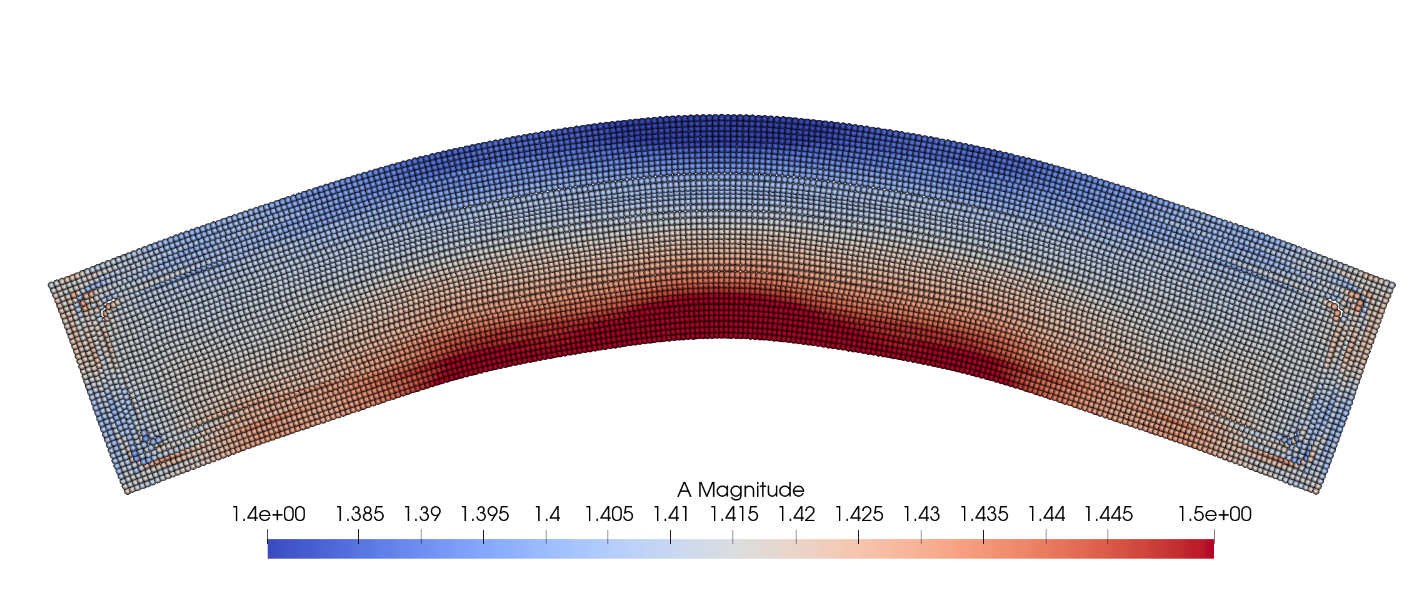
\includegraphics[width=0.85\linewidth]{plate1.png}
    \caption{For small deformations and large support radius it seems to 
    work at first.}
    \label{fig:plate1}
\end{figure}

\begin{figure}[H]
    \centering
    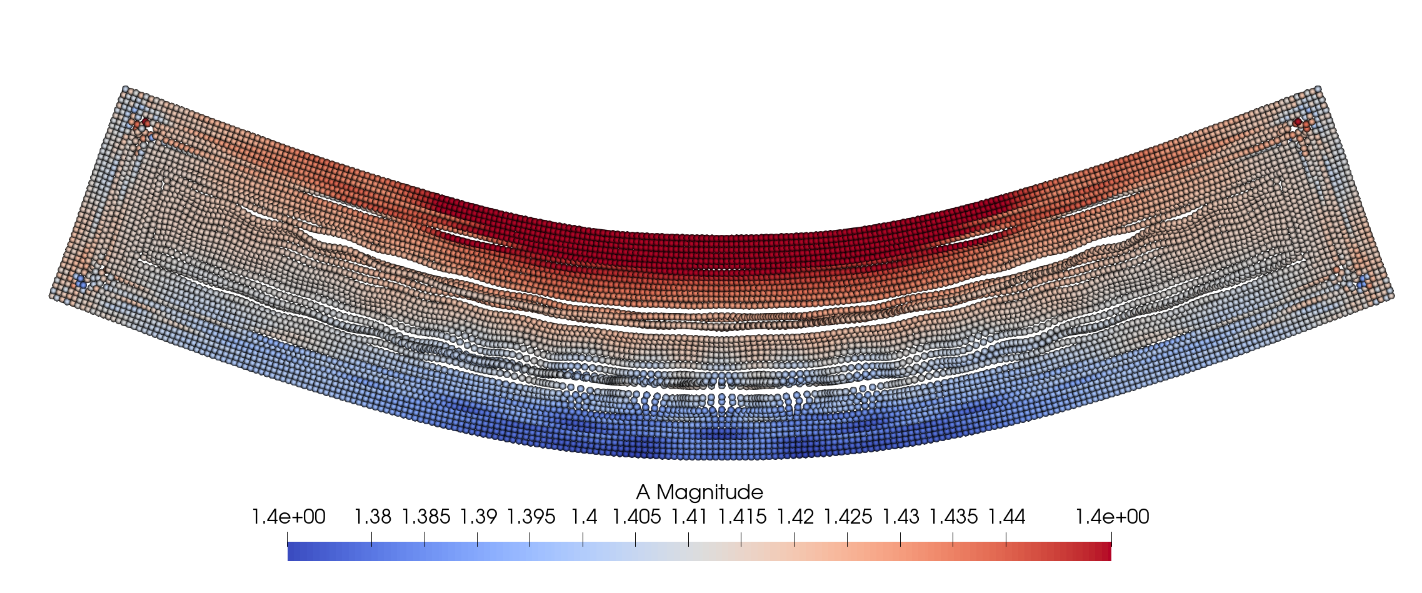
\includegraphics[width=0.85\linewidth]{plate2.png}
    \caption{However, even with support radius $h = 20dr$ (which is huge)
    the simulation becomes unstable after some time. 
    This does not seem to be tensile instability as the pressure is positive
    in the problematic places. It more has to do with this approximation 
    $\XX - \AA \xx \approx 0$.}
    \label{fig:plate2}
\end{figure}



\todo[inline]{TODO: Add the missing terms to the evolutoin equation for distorion to 
see what happens.}
\end{subsection}

%%% Bibliography
\bibliographystyle{abbrv}  % ama, nar, alpha, plain, chicago, abbrv, siam
\bibliography{library.bib}

\end{document}
